\chapter{Non-trusted environment issues}
We need to not trust an enviroment by default, becasue it can be compronised, and there are many ways to do so.

\section{Compromise causes}
\subsection{Node infection}
Nowadays, a node infection is obtained through a social engineering attack, that lead to the download of a compromise file/software.
\begin{itemize}[itemsep=0pt]
  \item Legitimate software containing malicious code (trojan horses) (a free version of paied software is alsways a good bait), social engineering, physical access, bug or configuration error exploitation (OS syscall, device driver, application, firmware and BIOS, browser ...)
  \item Backdoors creation, data stealing, hidden (or not so much) processes disruption, …
  \item Persistent unauthorized access to a system (as root - i.e. rootkits)
  \item Spyware (sensitive information collection)
  \item Ransomware (encryption of sensitive data)
\end{itemize}

\subsection{network injection}
\begin{itemize}[itemsep=0pt, topsep=0pt]
  \item nodes capable to read and write data while in transit, actors capable to "poison" routing mechanisms
  \item access and modification of network data flow, redirection versus illegitimate destination
  \item Sniffers and (growing) family of Man-in the-X  attacks
\end{itemize}

\subsection{supply chain attacks}
\begin{itemize}[itemsep=0pt, topsep=0pt]
  \item compromise of service, hardware, software of a third-party vendor or partner used (and trusted) by the target organization
  \item gain access to the target organization, inject unauthorized behavior
  \item infrastructure for update management
  \item
    \begin{itemize}[itemsep=0pt, topsep=0pt]
      \item e.g. SolarWind Orion Attack
      \item malicious code into software updates of Orion network monitoring platform.
      \item distributed to over 18,000 customers, including government agencies and large corporations.
    \end{itemize}
  \item libraries and dependencies
  \item hardware during manufacturing
  \item IT infrastructure management service
  \item ...
\end{itemize}
\subsection{Men at work} \label{sec:Mitx}

\subsubsection{man-in-the-middle}
An attacker secretly intercepts or alters communication between two unaware parties. \\Examples include \textbf{HTTP session hijacking}, where the attacker intercepts session cookies to impersonate a user, and \textbf{ARP table poisoning}, where ARP tables are altered for traffic redirection.

\subsubsection{man-in-the-browser}
Infection occurs in the browser to alter web pages or transactions.\\ An example is banking trojans like \textbf{ZEUS}, which modify online transactions.

\subsubsection{man-in-the-cloud}
This involves stealing credentials or tokens to access a user's cloud environment.\\ For example, the interception of a Google Drive OAuth token can allow access to the victim's files.

\subsubsection{man-in-the-mobile (MitMo)}
Mobile infection is used to intercept communication or two-factor authentication (2FA).\\ An example is ZitMo, which intercepts SMS and forwards them to a command and control (C\&C) server.

\subsubsection{man-in-the-disk}
This exploits vulnerabilities in handling external storage.\\ For instance, an attacker can modify temporary files stored on an external device.

\subsubsection{man-in-the-memory (MitMem - guest star)}
In this case, an attacker intercepts or modifies data while it is in RAM.\\ A notable example is fileless (stealth) malware.

\subsubsection{man-on-the-side}
An attacker observes and injects communication without modifying it.\\ An example is China's Great Cannon.

\subsubsection{man-at-the-end}
This type of attack compromises end-point communication.\\ For example, a keylogger infection can capture sensitive information.


\section{Advanced persistent threats (APT)}
\begin{itemize}[itemsep=0pt, topsep=0pt]
    \item \textbf{advanced}
    \begin{itemize}[itemsep=0pt, topsep=0pt]
        \item use of sophisticated techniques
        \begin{itemize}[itemsep=0pt, topsep=0pt]
            \item customised malware, zero day vulnerabilities, evasion stategies
        \end{itemize}
        \item targeted to specific victim
        \begin{itemize}[itemsep=0pt, topsep=0pt]
            \item high budget and expertise, careful preparation
        \end{itemize}
    \end{itemize}
    \item \textbf{persistent}
    \begin{itemize}[itemsep=0pt, topsep=0pt]
        \item Item compromise maintained for extended period
        \begin{itemize}[itemsep=0pt, topsep=0pt]
            \item possible escalation and infection diffusion
        \end{itemize}
        \item low-profile operation (during infection)
        \begin{itemize}[itemsep=0pt, topsep=0pt]
            \item stealth techniques, limited bandwidth usage, mimicking legitimate traffic
        \end{itemize}
    \end{itemize}
    \item \textbf{threat}
    \begin{itemize}[itemsep=0pt, topsep=0pt]
        \item highly skilled individual aiming strategic goals (espionage, foreign country intelligence, …)
    \end{itemize}
\end{itemize}


\subsection{APT Attack Process}

The Advanced Persistent Threat (APT) attack process consists of several key stages:

\subsubsection{Initial Intrusion}
The attacker gains access through a weak entry point, such as exploiting zero-day vulnerabilities or using spear phishing techniques to infiltrate the target system.

\subsubsection{Foothold Establishment}
Once access is gained, the attacker sets up persistent access by installing backdoors or infecting the system with (stealth) malware to maintain control over the compromised environment.

\subsubsection{Privilege Escalation}
The attacker escalates privileges to gain further control over the target system. This involves techniques like credential stealing or vulnerability exploitation.

\subsubsection{Lateral Movement}
The infection spreads across the target organization as the attacker moves laterally (like over different device/account with same/similar level of privilage), using stolen credentials (social eng.) or exploiting vulnerabilities to compromise additional systems.

\subsubsection{Goal Achievement}
The attacker eventually reaches their goal, which often involves data exfiltration or sabotaging critical systems.

\subsection{manupulation from the system owner}
If the system ownert is technical-savy, he can manipulate the system to hide the compromise, or to make it more difficult to detect, by installing modified application, compromised drivers or edit system calls.

\subsection{APTxx}

\textbf{APTxx} refers to organized hacker groups involved in advanced persistent threat (APT) activities. An example of such a group is \textbf{APT28}, also known as Fancy Bear.

\subsubsection{APT28 (Fancy Bear)}
APT28 is a \textbf{Russian state-sponsored group} that operates during Russian business hours and closely aligns with Russian government strategic interests, particularly in regions like the Caucasus. \\The group has been active since the mid-2000s, with documented operations dating back to at least 2008. APT28 targets a wide range of sectors, including aerospace, defense, energy, government, media, and dissidents, engaging in activities such as espionage, political influence, and cyberwarfare.

\paragraph{Notable Attacks:} In 2016, APT28 was responsible for the breach of the \textbf{Democratic National Committee} (DNC) during the U.S. presidential election. This attack led to the leakage of sensitive information with the intent of influencing the election outcome. \\Another major attack occurred in 2017 with the NotPetya ransomware, which was initially designed to target \textbf{Ukrainian institutions}. However, the malware spread globally, causing billions of dollars in damages.


\subsubsection{APT28 Typical Behavior}

APT28 targets a wide range of devices, including desktops, laptops, and mobile phones. It often employs \textit{(spear-)phishing} messages to direct victims to realistic websites for credential harvesting. 

\begin{itemize}[itemsep=0pt]
    \item APT28 registers domains that closely resemble legitimate organizations (e.g., \texttt{qov.hu.com} for the Hungarian government \texttt{gov.hu}).
    \item It uses URL-shortening services to obscure the true destination of malicious links.
\end{itemize}

In addition, APT28 delivers highly-realistic and targeted emails, often containing "weaponized" attachments such as \texttt{.docx} or \texttt{.pdf} files. \\They are alos used to implant custom malware, such as \textbf{X-Agent}, a multi-functional malware implant used for:
\begin{itemize}[itemsep=0pt]
    \item Data exfiltration,
    \item Keystroke logging
    \item Multiplatform operations (Windows, Linux, Android, and iOS).
\end{itemize}

After gaining initial access, APT28 actively seeks to harvest credentials through techniques like keylogging and central memory dumping. To evade detection, APT28 adopts various \textbf{evasion techniques}, including:
\begin{itemize}[itemsep=0pt]
    \item Malware code obfuscation,
    \item Use of compromised certificate signatures,
    \item \textit{Timestomping} (modifying timestamps), and
    \item Encrypted communication channels.
\end{itemize}

APT28 also engages in \textbf{lateral movement} within the compromised organization by exploiting harvested credentials. This lateral movement involves:
\begin{itemize}[itemsep=0pt]
    \item Remote Desktop Protocols (RDP),
    \item Windows Management Instrumentation Command-line (WMIC) and \texttt{PsExec} to execute commands on remote Windows machines, and
    \item \texttt{SSH} to connect to remote Linux systems.
\end{itemize}

At this point, APT28 escalates privileges by exploiting harvested credentials or vulnerabilities in the system. \bigskip

Finally, engages in \textbf{data exfiltration} using custom \textbf{Command-and-Control (C2)} communication frameworks, such as \textbf{Zebra C2}. The exfiltrated data may be optionally compressed, especially if large, and is transmitted via encrypted channels like \texttt{HTTPS}, \texttt{FTPS}, or even custom protocols.

Although primarily known for espionage, APT28 has also been involved in \textbf{destructive attacks}. These include the use of \textbf{wiper actions}, such as:
\begin{itemize}[itemsep=0pt]
    \item \textbf{KillDisk}, designed to destroy the master boot record, and
    \item Disk wiping tools, particularly in the energy sector.
\end{itemize}


\section{Trusted Environment}

The analysis must be performed in a \textbf{trusted environment}, as rootkits can \textbf{alter the normal behavior} of the operating system, making traditional tools unreliable.\\  
Rootkits are capable of \textbf{modifying file system utilities}, such as: \texttt{ls}, \texttt{cp}, \texttt{mv}, and other basic commands. \bigskip

Additionally, rootkits can intercept and \textbf{modify file system calls}. For example, they may intercept system calls like \texttt{open()}, \texttt{chdir()}, or \texttt{unlink()} to avoid displaying or acting on specific files, making it difficult to detect their presence.

\subsection{(example of) System Call Interception}
\begin{figure}[!ht]
    \centering
    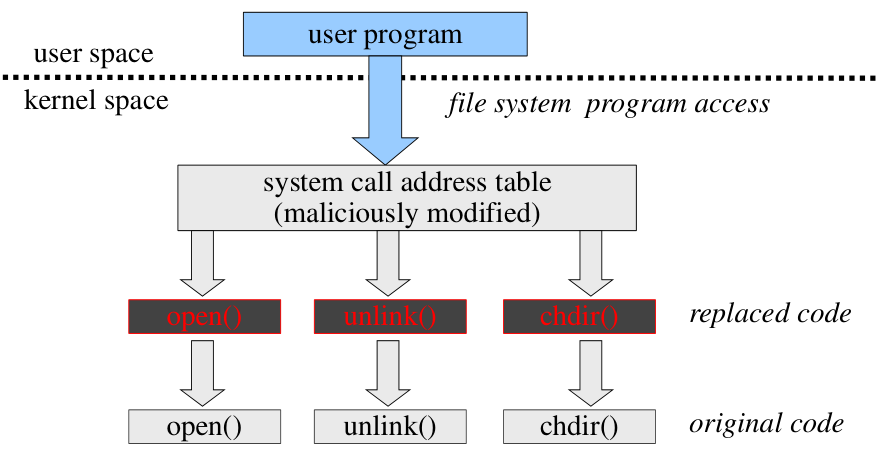
\includegraphics[width=0.5\textwidth]{img/sys_call_intercept.png}
    \caption{Example of System Call Interception}
    \label{fig:syscall_interception}
\end{figure}


\subsection{Examples of Linux system modification}

A common method of modifying a Linux system is through the use of \textbf{Loadable Kernel Modules (LKM)}. This concept is not unique to Linux and can be found in many other operating systems, such as kernel extensions in macOS or kernel-mode drivers in Windows.

An LKM can override the original system call (\textit{syscall}) function. The typical steps to achieve this include:

\begin{itemize}[itemsep=0pt]
    \item \textbf{Develop} a modified version of the system call function.
    \item \textbf{Modify} the system call table, which is an array of function pointers, to point to the new version of the function.
    \item If you want to \textbf{modify behavior}, you can re-implement the function with the desired changes.
    \item If you want to \textbf{add functionalities}, enrich the function with additional features and then call the original one to preserve its behavior.
\end{itemize}

This allows for either enhancing the system with new capabilities or subtly altering existing functionalities without being easily detected.
\begin{figure}[!ht]
    \centering
    \fboxsep=2mm%padding thickness
    \fboxrule=1pt%border thickness
    \fcolorbox{black}{white}{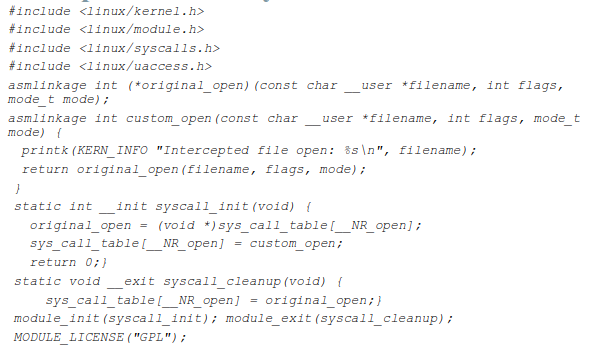
\includegraphics[width=0.6\textwidth]{img/linux_sys_modification.png}}
    \caption{Examples of Linux system modification}
    \label{fig:linux_sys_modification}
\end{figure}
